\chapter{Mission: Plant}

% played on a~2'x3' play area as

\emph{\emph{Plant} is a RECON+ mission in which the alliances attempt
  to destroy the campus physical plant using explosives chosen to
  incriminate their opponents, while preventing being similarly
  implicated themselves.}


\section{Play Area}
\vspace{-2\parskip}
\noindent\begin{stdminipage}{\linewidth-(2in+1.5em)}
\vspace{0pt}   
\noindent
Whichever player takes Deployment in the Initiative Roll chooses a
corner of the play area for their Deployment Zone, from which the
latter extends~12'' out.  The other player takes the diagonally
opposite corner as their Deployment Zone, again up to~12'' out.

A Network Terminal is placed at the center of the play area.

\section{Mission Rules}
As part of their deployment, both players secretly choose and record~3
scenery pieces wholly within~24'' of their opponent's Deployment Zone
corner as Vulnerable Infrastructure.  Each piece must have a footprint
of at least~4 square inches (e.g., a 2''x2'' square or~2.5'' diameter
circle).

In addition, as part of deployment, three troopers in each player's
army are given D-Charges.  This is public information as usual.
D-Charges already included in troopers' profiles may also be used.

\end{stdminipage}
\hfill
\begin{minipage}[t]{2in}\centering
\vspace{4pt}   
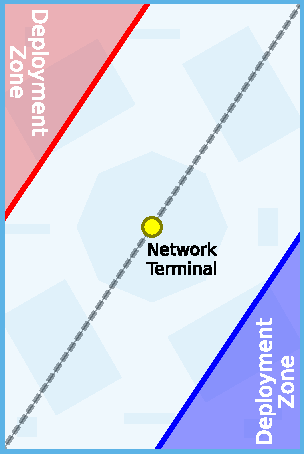
\includegraphics{maps/map-plant}
\end{minipage}

\section{Scoring}

Players may score up to~10 objective points via the following
conditions:
\begin{itemize}\shortlist
\item 1pt for each D-Charge you place on your chosen Vulnerable
  Infrastructure.
\item 1pt for each D-Charge you detonate on your chosen Vulnerable
  Infrastructure.
\item 3pts if you detonate D-Charges on all of your chosen Vulnerable
  Infrastructure simultaneously.

\item 1pt if the opposing Special Agent is in a Null state or
  eliminated at game end.
\end{itemize}

\vfill
\vbox to 0pt{}